\subsubsection{Rewrite}

Our sprint 1 code was messy and not well documented, so we did a full rewrite after the submission deadline. This was in the \verb|jottesen_test| folder, named so because it was initially a test of a new pathfinding algorithm. Similarly to \verb|sprint_1|, each robot type had its own class, along with several utility classes. We ended up (mostly) sticking with these utility classes for the rest of the competition, so we will describe them here.

\subsubsection{MapData}

This is really the core of ``what the bot knows''. It stores an array in memory, with one 32-bit int per tile on the map. Below is how we encoded the information in these bits:
\begin{center}
  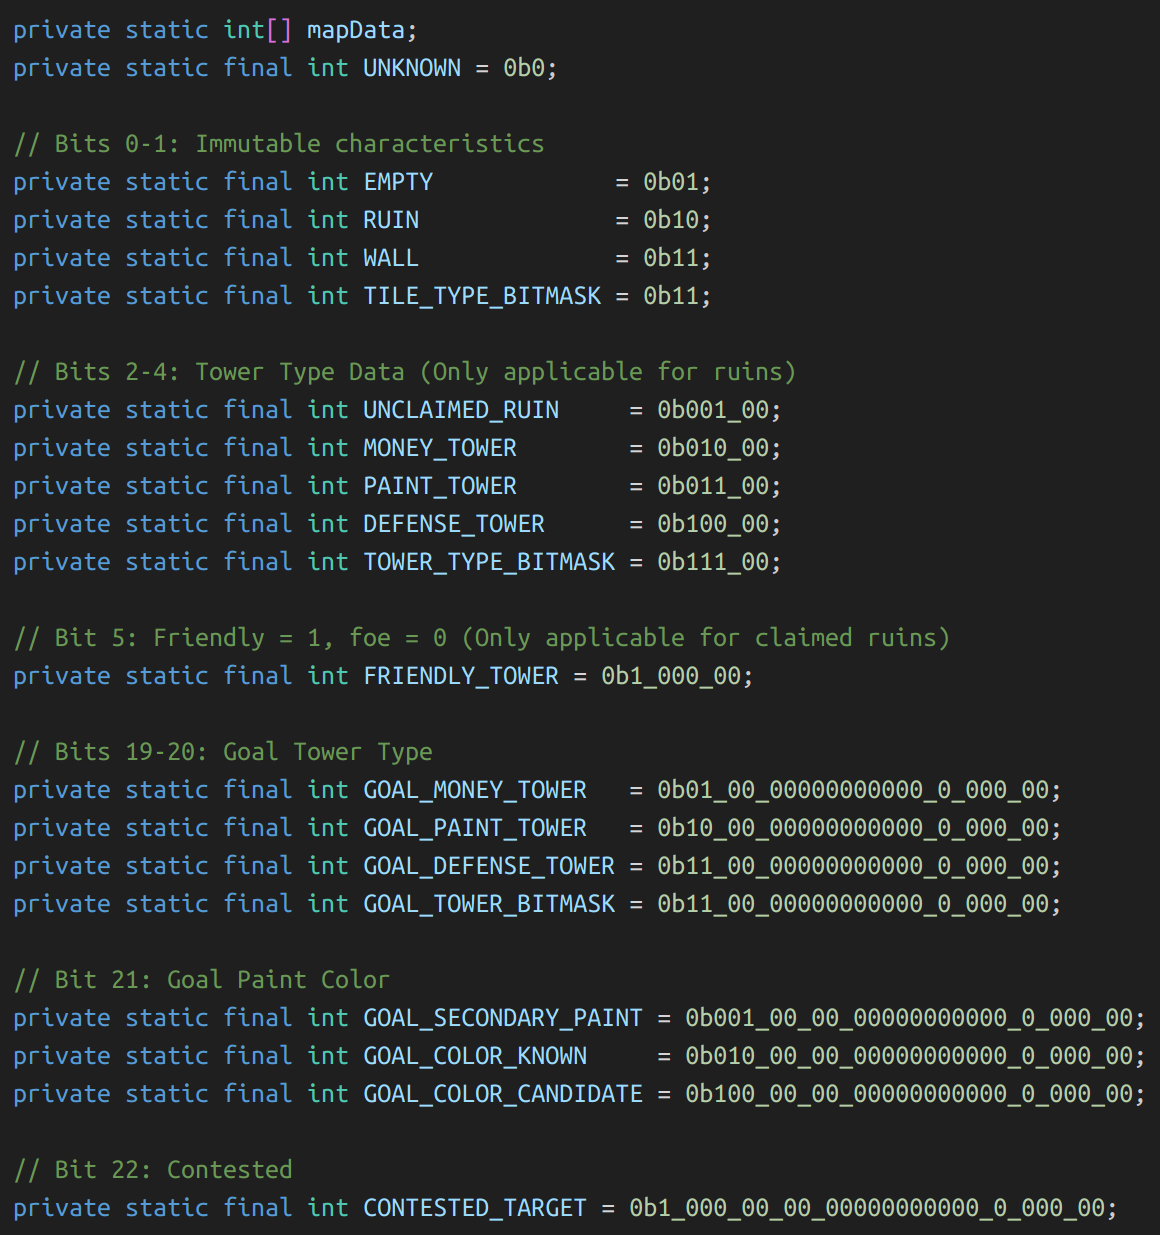
\includegraphics[scale=0.25]{images/mapData_bits.png}
\end{center}
We had plenty of bits left over, and many which were initially used and taken out. Upon spawning, each robot called \verb|MapData.updateAllVisible()| to load all known information about the immediate surroundings into the \verb|mapData| array. Each time the robot moved, it updated only the newly visible tiles. This was a bytecode compromise, since updating all the visible locations was expensive, but only updating newly visible leaves a blind spot around the robot. To help mitigate this, we also kept a list of the known ruins, and updated that list every turn.

\subsubsection{Painter}

We also created a \verb|Painter| class, which heavily relied on the \verb|MapData| class. The \verb|Painter| held the logic for which tiles should be painted, and what color should be used. It used the \verb|GOAL_*| bits from \verb|MapData| to encode these. Whenever we saw a ruin, we set these bits in the $5 \times 5$ area around it. We later did the same with SRPs\footnote{This bot did not bother to paint SRPs, but still heavily outplayed the previous version}. This really streamlined our painting logic, and we didn't have to worry about checking the correct color each time.

\medskip

We also put logic for moppers here, but our moppers were terrible so it isn't really important to discuss. At this point, we still didn't have splashers.

\subsubsection{Communication}

We added the groundwork for our future communication class, however it was not used at all in this iteration. We wrote functions to communicate map symmetry, but did not use them until much later in the competition.

\subsubsection{Pathfinding}

This class was one of the big upgrades of the rewrite\footnote{It was honestly a waste of time since we ended up scrapping it later. It used too much bytecode and was too buggy.}. In the initial bot, we used a pure BugNav algorithm from a previous year, as mentioned previously. This worked, but was inefficient at times. Since we stored the map internally, we could simulate doing BugNav, but have the bot actually take shortcuts.

\medskip

The core idea was that the bot would have some goal target that it was trying to move towards. The algorithm is loosely described below:
\begin{enumerate}
  \item Simulate greedy movement towards the target on the internal \verb|MapData| array. If you hit either the target or an unknown tile, return and follow that path.
  \item If you hit an obstacle, simulate BugNav until you make it past, or you hit an unknown tile.
  \item Repeat the algorithm on the result of the above BugNav.
\end{enumerate}
We managed the target destinations by creating a fixed buffer \verb|Stack| class. Whenever we needed a checkpoint target (found by the BugNav step), we would push it onto the stack. When we reached that target, we popped it off and recalculated the path to the next target. Another useful optimization we used in pathfinding was caching and pre-calculating moves. This let us calculate several moves in advance without wasting a ton of bytecode on recalculations.

\medskip

The main reasons this failed were because of high bytecode cost, greedy search instead of BFS, and bad handling of the case of maximum stack depth of locations. It would outperform our old algorithm in ``easy'' pathfinding scenarios, but would often unpredictably get stuck on the harder situations. Traditional BugNav was a more reliable solution.

\subsubsection{Opening Rush}

Up until this point, we hadn't really considered any type of coordinated effort. Our entire goal was just to build up economy, and if you see any enemies, try and beat them. This is the point we started to consider higher level strategy, so we made a \verb|sprint_2| bot to test our changes against the previous \verb|jottesen_test| and make sure we were in fact making improvements.

\medskip

Rush was very strong at this point of the competition, since two initial soldiers could fully take out an opponent tower. We decided to fight fire with fire, and Andrew meticulously coded a coordinated rush strategy. Each tower would spawn two soldiers, and using the map symmetry, we sent each pair to a different candidate enemy tower location. However, if the soldiers found an uncontested ruin\footnote{A ruin with no enemy paint blocking the pattern} on the way to the enemy tower, they would try to capture the ruin. Until the soldiers finished the first ruin, they were in ``opening mode'', meaning if their current ruin became contested, they continued the rush.

\medskip

If the soldiers successfully took out an enemy tower, we assumed that the enemy had done the same to us, and the soldiers went into pure survival mode to try and help us win on tiebreakers in case all towers were taken out. This was not a problem if the opponent didn't rush us, since our towers would just produce more units, and these soldiers were low enough on paint and health after fighting the enemy tower that they wouldn't be able to make it back or do anything useful.

\subsubsection{GoalManager}

The last big change we made before Sprint 2 was introducing the \verb|GoalManager| class. We previously were storing the goal location as a single \verb|MapLocation| and the type as an enum. However, this lead to many problems. Often, ruins would be abandoned when robots went back to get their paint refilled, since they were the only robot that knew it was in progress. After refilling paint, they would act as if they were a new soldier.

\medskip

We decided to use a stack for the goals, giving robots a lot more choice in their intended actions on goals. They could either 